\section{Obtención de nombres de profesores} \label{nomProfesores}

Antes de iniciar la simulación de las solicitudes hechas (elección de materia y de horario), primero obtuvimos información de los profesores. Guardamos dicha información en la matriz \textit{mat\_nom\_prof\_total}, la cual tiene 2 columnas. En la primer columna se tienen los nombres de todos los profesores que han impartido clase desde el semestre 2015-1 hasta el 2020-1. Dichos nombres los obtuvimos de la matriz \textit{m\_grande\_2015}. En la segunda columna de la matriz, se tiene un $1$ si el profesor es de tiempo completo y un $0$ si es de asignatura.

En las siguientes subsecciones veremos cómo llenamos la segunda columna de la matriz \textit{mat\_nom\_prof\_total} y cómo hicimos la limpieza de los nombres de los profesores.

\subsection{Profesores de tiempo completo}

Para llenar la segunda columna de la matriz \textit{mat\_nom\_prof\_total} ingresamos a la página \url{http://www.matematicas.unam.mx/index.php/nosotros/profesores-de-tiempo-completo} del Departamento de Matemáticas. Con la aplicación \textit{SelectorGadget} seleccionamos el vector con el nombre de los profesores de tiempo completo. En la \figurename{~\ref{profTC_SelectorGadget}} podemos ver el código CSS que utilizamos para obtener los datos en \textit{R}. También observamos que se seleccionaron 94 profesores.

\begin{figure}[H]
\centering
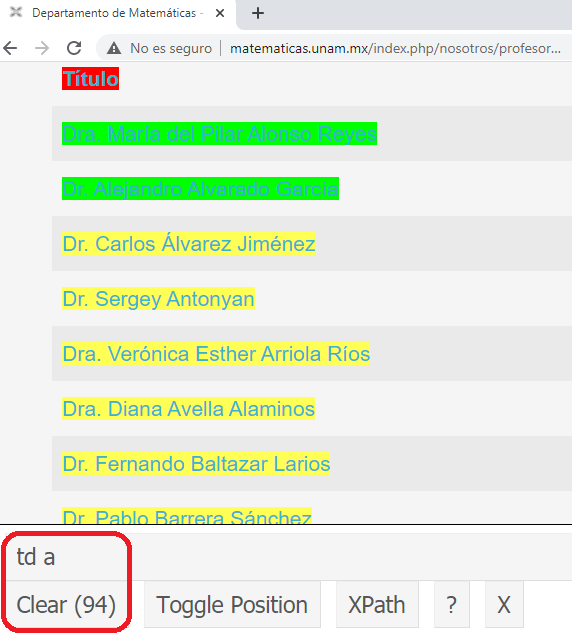
\includegraphics[scale = 0.6]{profesores_TC_SelectorGadget} %width=\textwidth
\caption[\textit{Profesores de tiempo completo: SelectorGadget}]{\textit{Profesores de tiempo completo obtenidos con la aplicación SelectorGadget: Muestra la selección de profesores de tiempo completo con la aplicación SelectorGadget. Se puede ver el código CSS utilizado en R.}}\label{profTC_SelectorGadget}
\end{figure}

Al extraer la información en \textit{R} obtuvimos un vector con 94 entradas. En la \figurename{~\ref{profTC_sinLimpiar}} podemos ver los primeros 20 valores del vector. Notamos que cada entrada del vector inicia con los caracteres $\backslash n \backslash t \backslash t \backslash t \backslash t \backslash t \backslash t \backslash t$. Estos caracteres, en la presentación final de la página de internet, indican un salto de línea y las tabulaciones o espacios que se tienen de izquierda a derecha.

\begin{figure}[H]
\centering
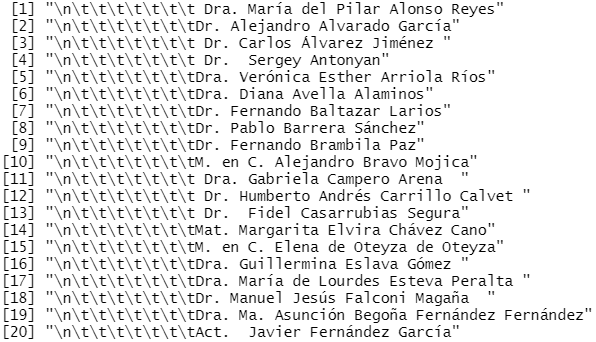
\includegraphics[scale = 0.7]{profesores_TC_sinLimpiar} %width=\textwidth
\caption[\textit{Vector de profesores de tiempo completo}]{\textit{Vector de profesores de tiempo completo: Se observan las primeras 20 entradas del vector obtenido con la aplicación SelectorGadget al dar click en un profesor de tiempo completo.}}\label{profTC_sinLimpiar}
\end{figure}

Limpiamos los datos para obtener un vector que sólo tuviera los nombres de los profesores, sin su título. Eliminamos el título porque en los horarios publicados en las páginas de la FC sus nombres no tienen título. También eliminamos los espacios finales que había en algunos nombres.

De esta manera obtuvimos el vector con el nombre de los profesores de tiempo completo del Departamento de Matemáticas. Dicho vector lo comparamos con la primer columna de la matriz \textit{mat\_nom\_prof\_total}, cuando los nombres coincidieron, pusimos un $1$ en el renglón correspondiente.

Al limpiar los datos encontramos 11 nombres que analizamos de manera particular porque no aparecía el $1$ en su respectivo renglón. Encontramos que no aparecía la información necesaria en la matriz \textit{mat\_nom\_prof\_total} por diferencias en los nombres. Encontramos diferencias por acentos, por mayúsculas y por nombres incompletos. En la \tablename{~\ref{DifNomProfTC}} vemos los nombres que aparecen en las páginas de la FC comparados con los que aparecen en la página del Departamento de Matemáticas.

\begin{table}[h]
\centering
\resizebox{\textwidth}{!}{%
  \begin{tabular}{|c|c|}
  \hline 
  \textbf{Nombre en páginas de la FC} & \textbf{Nombre en página del Depto. de Matemáticas} \\ 
  \hline 
  Alejandro Ricardo Garciadiego Dantan & Alejandro Ricardo Garciadiego Dantán \\ 
  \hline 
  Edith Corina Sáenz Valadez & Edith Corina Sáenz Valadéz \\ 
  \hline 
  Emilio Esteban Lluis Puebla & Emilio Lluis Puebla \\
  \hline 
  Guillermo Javier Francisco Sienra Loera & Guillermo Sienra Loera \\
  \hline 
  María Asunción Begoña Fernández Fernández & Ma. Asunción Begoña Fernández Fernández \\ 
  \hline 
  María Concepción Ana Luisa Solís González-Cosío & Ana Luisa Solís González Cosío \\ 
  \hline
  María Isabel Puga Espinosa & Isabel Puga Espinosa \\ 
  \hline 
  María Lourdes Velasco Arreguí & María de Lourdes Velasco Arregui \\ 
  \hline 
  Mucuy-Kak del Carmen Guevara Aguirre & Mucuy-kak del Carmen Guevara Aguirre \\ 
  \hline 
  Oscar Alfredo Palmas Velasco & Óscar Alfredo Palmas Velasco \\ 
  \hline 
  Úrsula Xiomara Iturrarán Viveros & Úrsula Iturrarán Viveros \\ 
  \hline 
  \end{tabular}
} 
\caption[\textit{Diferencias en nombres de profesores de tiempo completo}]{\textit{Diferencias en nombres de profesores de tiempo completo: Se muestran los 11 nombres de los profesores de tiempo completo que se analizaron de manera individual.}}\label{DifNomProfTC}
\end{table}

\subsection{Profesores de asignatura}

Al llenar la matriz \textit{mat\_nom\_prof\_total} con los nombres de los profesores vimos que la dimensión de dicha matriz es $1387 \times 2$. Por lo que tenemos 1387 nombres de profesores de los cuales 94 son profesores de tiempo completo. En esta subsección explicaremos cómo hicimos la limpieza de los nombres de los profesores de asginatura. Es decir los 1293 nombres que nos falta por analizar.

*** EXPLICAR LIMPIEZA DE LOS NOMBRES DE PROFESORES DE ASIGNATURA CON FUNCIÓN stringsim***









Algunas notas a considerar de esta matriz son:
  
  \begin{itemize}
\item[-] Hay profesores que se repiten por diferencia de acentos, como: \textit{César Alejandro Arellano Ruíz, Luis Eduardo García Hernández}.

\item[-] Hay profesores que se repiten por tener a lado el nombre de los ayudantes, como: \textit{Fermín Alberto Viniegra Heberlein, Edgar Vázquez Luis}.

\item[-] Puede haber profesores que ya no impartan clases en la FC.
\end{itemize}
